\documentclass[letterpaper,12pt]{article}
%\documentclass[journal]{IEEEtran}
\usepackage{amssymb,amsmath}
\usepackage{bookman}
\usepackage{url}
\usepackage{graphicx}
\usepackage{lmodern}
\usepackage{microtype}
\usepackage[font=small,labelfont=bf]{caption}
\usepackage[numbers]{natbib}
\usepackage[pdftex,
            pdfauthor={Carlos Rueda},
            pdftitle={LPC Based Analysis and Clustering on Humpback Whale Vocalizations},
            colorlinks=true,allcolors=black]{hyperref}

%\hypersetup{backref, pdfpagemode=FullScreen, colorlinks=true}

\addtolength{\hoffset}{-1.5cm}
\addtolength{\textwidth}{3.5cm}
%\addtolength{\voffset}{2cm}
\setlength{\parskip}{1ex plus 0.5ex minus 0.2ex}

%No hyphenation:
\usepackage[none]{hyphenat}
%\tolerance=200
\setlength{\emergencystretch}{2em}


\DeclareMathOperator*{\argmax}{argmax}
\DeclareMathOperator*{\argmin}{argmin}

\newcommand{\bA}{\ensuremath{\mathbf{A}}}
\newcommand{\ba}{\ensuremath{\mathbf{a}}}
\newcommand{\bb}{\ensuremath{\mathbf{b}}}
\newcommand{\bc}{\ensuremath{\mathbf{c}}}
\newcommand{\bs}{\ensuremath{\mathbf{s}}}
\newcommand{\bx}{\ensuremath{\mathbf{x}}}
\newcommand{\br}{\ensuremath{\mathbf{r}}}
\newcommand{\bo}{\ensuremath{\mathbf{o}}}
\newcommand{\bC}{\ensuremath{\mathbf{C}}}
\newcommand{\bR}{\ensuremath{\mathbf{R}}}
\newcommand{\bq}{\ensuremath{\mathbf{q}}}
\newcommand{\bv}{\ensuremath{\mathbf{v}}}
\newcommand{\bw}{\ensuremath{\mathbf{w}}}


\title{LPC Based Analysis and Clustering\\
 on Humpback Whale Vocalizations}
\author{Carlos A. Rueda\\
\\
(draft)}
%\date{}

\begin{document}
    \maketitle

    \begin{abstract}

        This document provides some basic background relevant to the
        clustering experiments performed on whale vocalizations
        reported at \url{https://github.com/ecoz2/ecoz2-whale-cb}.
        The processing of the signal is based on linear predictive coding.
        In each experiment, LPC analysis is applied on given whale sound files
        to generate corresponding training vectors for clustering.
        The training vector space is then clustered using a non-Euclidian
        version of K-means where an LPC-based distance function is used.
        Codebooks of incremental size are generated while capturing some metrics
        for evaluation and visualization, including average distortion as a
        function of codebook size;
        cluster cardinality and distortion for specific codebook sizes;
        and minimum distortion for each training vector to support visualization
        of cluster shapes based on the reflection coefficients associated
        with the prediction coefficients.

    \end{abstract}

    \section{Linear Predictive Coding}\label{sec:linear-predictive-coding}

    Linear predictive analysis is a widely used techique in speech processing~\citep{Rabiner:Schafer:2007,Parsons:87}.
    \
    On humpback whale vocalizations, \citep{Howard:2018} is a recent and
    relevant reference in that not only includes LPC as part of their analysis,
    but also, more generally, investigates the sub-unit structure of song units,
    which is one of the core motivations for the experiments in our work.

    In what follows we introduce some minimal LPC background but hopefully
    sufficient to articulate the main aspects explored in the reported experiments
    at \url{https://github.com/ecoz2/ecoz2-whale-cb}.
    Further details can be found in the references.

    Let $\bs = [ s_1, s_2, \ldots, s_L ]$
    be the discrete signal representing a certain whale vocalization or
    series of vocalizations.
    \
    To obtain a more compact representation of the signal, yet not loosing
    significant information,
    we use \textit{linear predictive coding} (LPC) analysis.
    \
    This analysis is applied on consecutive, overlapping time windows where
    the signal in each window is assumed to be approximately stationary
    (i.e., statistics within the window do not change as a function of time).
    \
    Let $T$ be the number of windows extracted from $\bs$,
    and $\bx = [ x_1, x_2, \ldots, x_N ]$ denote one of such windows.
    \
    The core idea in LPC analysis is to estimate each sample value $x_n$
    as a linear combination of a number of previous sample values:

    \[
        \hat{x}_n = \sum\limits_{i=1}^{P} a_i x_{n-i}
    \]
    where $P$ is the \textit{order of the prediction}.
    \
    So, the  error at the $n$-th sample is:
    \[
        e_n = x_n - \hat{x}_n
            = x_n - \sum\limits_{i=1}^{P} a_i x_{n-i}
    \]
    and the goal is to find the $a_i$ coefficients that minimize the
    squared error over the window:
    \[
        E = \sum\limits_n e^2_n
          = \sum\limits_n ( x_n - \sum\limits_{i=1}^{P} a_i x_{n-i} )^2
    \]

    It is possible to solve this problem with a variety of methods and
    depending on particular signal characteristics (e.g., voiced or unvoiced).
    The software\footnote{
        \url{https://github.com/ecoz2/ecoz2},
        developed as part of~\citep{Rueda:1993}.
    }
    used in our experiments apply the \textit{autocorrelation method}
    as described in~\citep{Parsons:87}.
    \
    The details are out of the scope of this document but we will note that
    this error can be expressed in matrix form as:
    \
    \begin{equation}
        E = \ba^\prime \bR \ba  \label{eq-E-quadratic}
    \end{equation}
    where $^\prime$ denotes the transpose operation and
    $\bR$ is the the autocorrelation matrix of window $\bx$.
    This expression is used below as the basis to measure the
    distance between two prediction vectors.

	\begin{figure}[!ht]
		\centering
		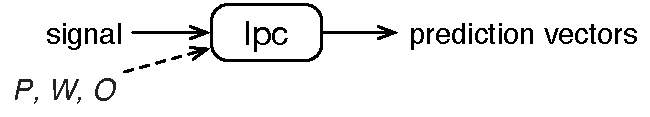
\includegraphics[width=0.4\textwidth]{lpc.pdf}
		\caption{
		The LPC analysis step applied on a signal resulting in a number of prediction vectors.
        $P$ is the order of prediction, and $W$ and $O$ are the window size and offset in ms.
		}
		\label{fig:lpc-step}
	\end{figure}

    So, by applying LPC analyis on each of the windows $\bx$ from the
    input signal we obtain the corresponding prediction coefficients,
    $\ba = [ a_1, a_2, \ldots, a_P ]$.
	Fig.\,\ref{fig:lpc-step} is a schematic of this step.

    \section{Clustering}\label{sec:clustering}

    The set of all LPC vectors extracted from the input signal
    will comprise the training set for clustering.
    We closely follow Juang et al~\citep{Juang-etal:82}
    for the implementation of the clustering algorithm as well as in terms of
    evaluation based on distortion performance.

    A core operation required for clustering is measuring the distance or
    distortion $d(\ba,\bb)$ between two LPC vectors $\ba$ and $\bb$.
    Since the vectors are coming from linear predictive analysis,
    we use a measure based on the prediction error itself according
    to (\ref{eq-E-quadratic}).
    \
    More specifically, noting that (\ref{eq-E-quadratic}) is the minimum prediction error
    found for a particular window $\bx$ from which $\ba$ was obtained, we can also
    perform a similar calculation, still using the same autocorrelation matrix $\bR$
    for $\bx$, but involving any other prediction vector $\bb$:

    \begin{equation}
        E_\bb = \bb^\prime \bR \bb   \label{eq-E-quad-b}
    \end{equation}

    Since $E_\bb \ge E_\ba$, we can define the distorion measure as:

    \begin{equation}
        \begin{array}{rcl}
            d(\ba,\bb) &=& E_\bb / E_\ba - 1  \label{eq-dist0}
        \end{array}
    \end{equation}

    In part because the autocorrelation matrix $\bR$ is symmetric and \textit{Toeplitz},\footnote{
        \url{https://en.wikipedia.org/wiki/Toeplitz_matrix}
    }
    it can be shown that the prediction error given in (\ref{eq-E-quad-b})
    can be expressed as the scalar product:

    \begin{equation}
        E_\bb = \br_\bx[0] \br_\bb[0] + 2 \sum_{p = 1}^P \br_\bx[p] \br_\bb[p] \label{eq-Eb}
    \end{equation}
    where
    $\br_\bx$ is the autocorrelation sequence of $\bx$
    and
    $\br_\bb$ is the autocorrelation sequence of the prediction vector $\bb$.
    \
    Using this in (\ref{eq-dist0}) we get~\citep{Juang-etal:82}:

    \begin{equation}
        d(\ba,\bb) = \frac{\br_\bx[0]}{E_\ba} \br_\bb[0] + 2 \sum_{p = 1}^P \frac{\br_\bx[p]}{E_\ba} \br_\bb[p]
                     - 1
                     \label{eq-dist}
    \end{equation}

    With the distortion measure function now established,
    let us now proceed with the clustering step.
    \
    Let $\bA = [ \ba_1, \ba_2, \ldots, \ba_T ]$
    be the set of prediction coefficient vectors that we want to cluster.
    The clustering method used here is a variant of the $K$-means algorithm~\citep{LBG:80,Parsons:87}.
    \
    With $\bA$ as input and a threshold parameter $\epsilon$ used as a convergence criterium
    (i.e., a change in average distortion --see below-- less than this threshold stops the iterative
    refinement of the codebook),
    the method generates codebooks of incremental size.
    For a given size $K$, the method finds the set of centroids
    $\bC = [ \bc_1, \bc_2, \ldots, \bc_K ]$
    that best represent the vector space associated with the training
    set according to the distortion measure, that is,
    one that minimizes the average distortion:
    \begin{equation}
        D_K = { \frac{1}{T} } \sum_{\ba \in \bA} \min\limits_{k=1}^{K} d(\ba,\bc_k) \label{eq-Dk}
    \end{equation}

    The method first creates a
    codebook of size $K=2$ using $K$-means.
    Once the average distortion is sufficiently small for this size
    according to the $\epsilon$ parameter,
    the codebook is doubled in size (via splitting each centroid into two)
    and the $K$-means algorithm is performed on the new size $K=4$.
    This procedure is repeated until a maximum codebook size is reached.
    \
    Fig.\,\ref{fig:clustering-step} illustrates the clustering step.

    \begin{figure}[!ht]
        \centering
        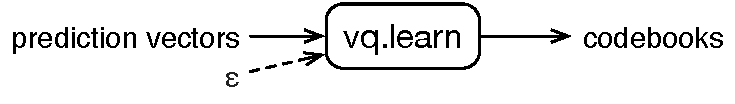
\includegraphics[width=0.45\textwidth]{clustering.pdf}
        \caption{
        The clustering step applied on a set of prediction vectors resulting in a
        number of codebooks of incremental size.
        }
        \label{fig:clustering-step}
    \end{figure}

    Codebooks typically become the basis to subsequently perform
    \textit{vector quantization}\footnote{
        Vector quantization basically consists in mapping any given $P$-order
        vector $\ba$ (not necessarily from the training set)
        to the index $k_\ba$ in a codebook $\bC$ of size $K$ such that
        $k_\ba = \argmin\limits_{k=1}^{K} d(\ba, \bc_k)$.
    },
    which is used in a variety of applications.
    Here, we are mainly focused on the clustering process itself and
    the inspection and evaluation of the generated codebooks.

    \subsection{Codebook evaluation}\label{subsec:codebook-evaluation}

    The evaluation in our experiments is of an \textit{internal}\footnote{
        \url{https://en.wikipedia.org/wiki/Cluster_analysis\#Evaluation_and_assessment}
    } nature.
    As a function of codebook size $K$, we capture and inspect the following values:

    \begin{itemize}
        \item Average (intra-cluster) distortion ${D_K}$, as defined in (\ref{eq-Dk});

        \item $\sigma$-ratio, the ratio between the inter-cluster and intra-cluster
            average distortions~\citep{Rabiner:Levinson:Sondhi:1983}:
            \[
                \sigma_K = \frac{ \frac{1}{K} \sum\limits_{i=1}^{K} \frac{1}{K-1} \sum\limits_{j=1}^{K} d(\bc_i, \bc_j) }
                           {D_K};
            \]

        \item \textit{Inertia} (``within-cluster sum-of-squares criterion''),
             definition adapted from~\citep{scikit-inertia}:
            \[
                \mathbf{inertia}_K = \sum_{\ba \in \bA} \min\limits_{k=1}^{K} d(\ba,\bc_k)^2. \label{eq-inertia}
            \]
    \end{itemize}

    Fig.\,\ref{fig:cb_evaluation}, taken from one of the reported experiments,
    shows a typical plot of these values as a function of codebook size.
    \begin{figure}[!ht]
        \centering
        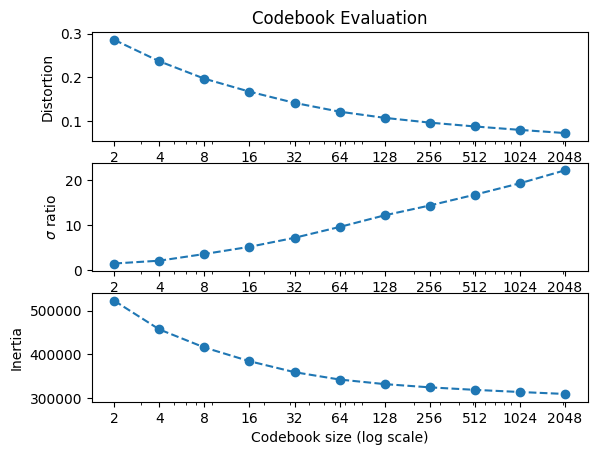
\includegraphics[width=0.65\textwidth]{../6_good_songs/cb_evaluation.png}
        \caption{
        A plot of average distortion, $\sigma$-ratio, and inertia.
        }
        \label{fig:cb_evaluation}
    \end{figure}

    For each cluster we also track its cardinality
    (number of training vectors in each cluster)
    and average distortion~\citep{Rabiner:Levinson:Sondhi:1983}.
    \
    Fig.\,\ref{fig:cb_cards_dists_scatter} shows a resulting scatter plot
    from one of the experiments with a codebook of size $M=1024$.
    \begin{figure}[!ht]
        \centering
        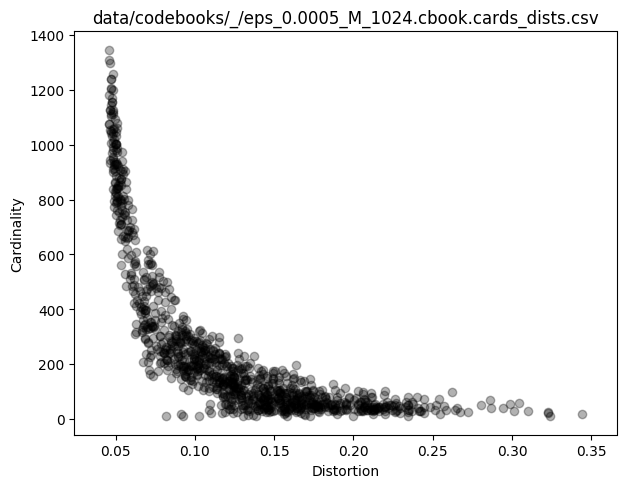
\includegraphics[width=0.6\textwidth]{../6_good_songs/cb_cards_dists_scatter.png}
        \caption{
        A typical distortion vs. cardinality scatter plot
        (the greater the cluster distortion, the lower its cardinality).
        }
        \label{fig:cb_cards_dists_scatter}
    \end{figure}

    \subsection*{Cluster visualization}

    \begin{figure}[!ht]
        \centering
        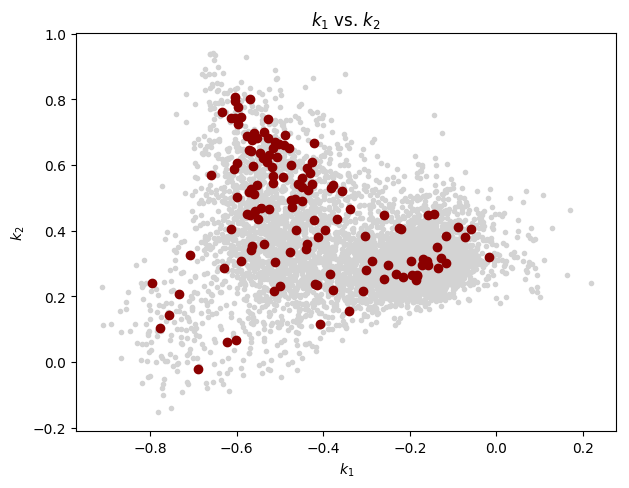
\includegraphics[width=0.6\textwidth]{../HBSe_20170128T231621/cb_kk_training_8000_codebook_128.png}
        \caption{
        $k_1$-$k_2$ scatter plot showing values from training vectors (gray dots) and
        codebook centroids (red dots).
        Codebook size $M=128$.
        }
        \label{fig:cb_kk_training_8000_codebook_128}
    \end{figure}

    Instead of visualizing the space of the prediction coefficient vectors $\ba$
    directly, we follow~\citep{Juang-etal:82} to look into the
    corresponding \textit{reflection coefficient} vector space.
    \
    Fig.\,\ref{fig:cb_kk_training_8000_codebook_128}
    plots the first two reflection coefficients, $k_1$ and $k_2$,
    taken from the training vector set as well as from the resulting codebook ($M=128$).
    \
    A similar plot but with the first three reflection coefficients is shown
    in Fig.\,\ref{fig:cb_kkk_training_8000_codebook_1024}.
    \begin{figure}[!ht]
        \centering
        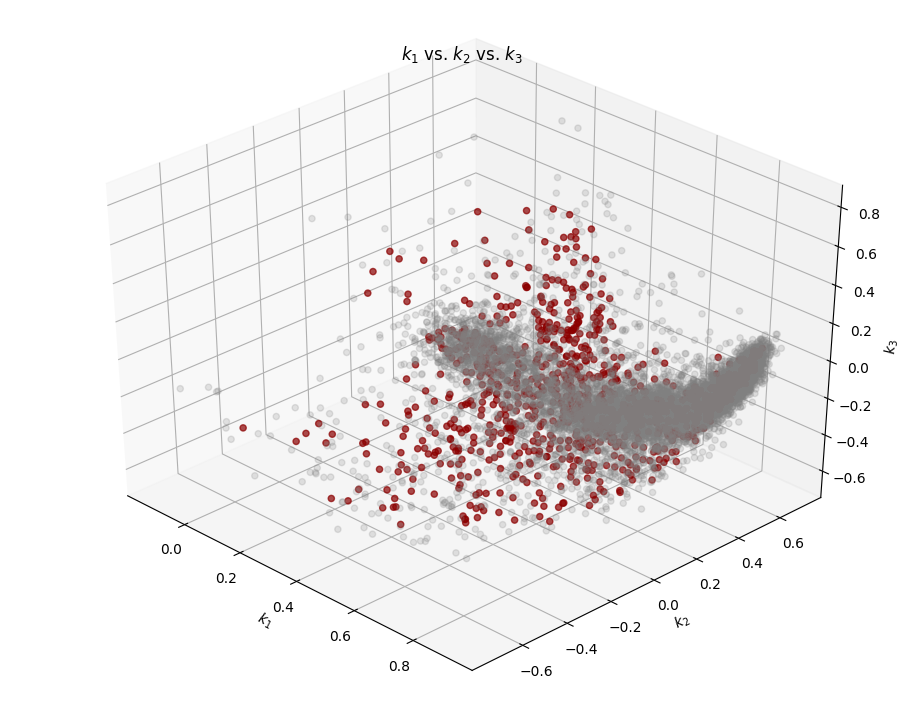
\includegraphics[width=0.7\textwidth]{../MARS_20161221_000046_SongSession_16kHz_HPF5Hz/cb_kkk_training_8000_codebook_1024.png}
        \caption{
        $k_1$-$k_2$-$k_3$ scatter plot showing values from training vectors (gray dots) and
        codebook centroids (red dots).
        Codebook size $M=1024$.
        }
        \label{fig:cb_kkk_training_8000_codebook_1024}.
    \end{figure}


    \clearpage
    \bibliographystyle{unsrt}
    \bibliography{lpckw}

\end{document}

